\begin{tikzpicture}[x=1cm,y=1cm,font=\sffamily\footnotesize,
  panel/.style={draw=black!15,rounded corners=2pt,fill=black!2},
  action/.style={draw=teal!65!black,rounded corners=2pt,fill=teal!7,align=center,text width=2.5cm,minimum height=.55cm},
  arrow/.style={-{Stealth[length=1.8mm]},thick,draw=teal!70!black}]
\draw[panel] (0,0) rectangle (5,4.2);
\draw[panel] (5.35,0) rectangle (10.85,4.2);
\draw[panel] (11.2,0) rectangle (17.2,4.2);
\node[anchor=west,font=\sffamily\bfseries\small] at (.22,3.88) {1\quad See the initial evidence};
\node[anchor=west,font=\sffamily\bfseries\small] at (5.57,3.88) {2\quad Choose how to look};
\node[anchor=west,font=\sffamily\bfseries\small] at (11.42,3.88) {3\quad Decide with evidence};
\node[align=center,text width=4.6cm] at (2.5,3.25) {Claim: A and B are the same physical chair.};
\node at (1.3,1.75) {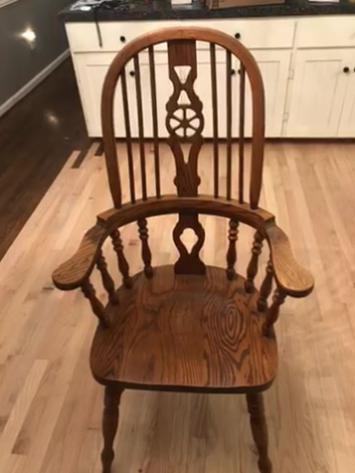
\includegraphics[height=1.95cm,width=1.95cm,keepaspectratio]{figures/chair-a.jpg}};
\node at (3.75,1.75) {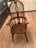
\includegraphics[height=1.95cm,width=1.95cm,keepaspectratio]{figures/chair-b-preview.jpg}};
\node at (1.3,.54) {A: current view};
\node at (3.75,.54) {B: preview};
\node[action] (local) at (7.0,2.95) {Inspect / crop / compare};
\node[align=center,text width=2.4cm,text=black!65,font=\sffamily\scriptsize] at (9.45,2.95) {Re-examine\\released pixels};
\node[action] (request) at (7.0,1.53) {Request object,\\time and view};
\node (newview) at (9.6,1.65) {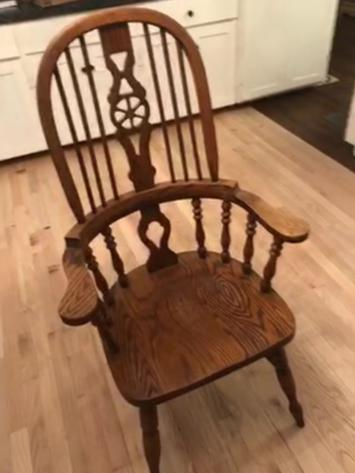
\includegraphics[height=1.55cm,width=1.25cm,keepaspectratio]{figures/chair-a-new.jpg}};
\node[font=\sffamily\scriptsize,align=center] at (9.6,.53) {Recorded view\\if available};
\draw[arrow] (5,2.65) -- (5.35,2.65);
\draw[arrow] (local.east) -- (8.65,2.95);
\draw[arrow] (request.east) -- (8.95,1.53);
\draw[arrow] (10.85,2.65) -- (11.2,2.65);
\node[draw=teal!65!black,fill=teal!7,rounded corners=2pt,align=center,text width=5.1cm,minimum height=.65cm] at (14.2,3.05) {Supported\quad Refuted\quad Need more evidence};
\node[align=left,text width=5.1cm] at (14.2,1.82) {
  \textbf{Support:} cover every subclaim.\\[3pt]
  \textbf{Refute:} cite a decisive counterexample.\\[3pt]
  \textbf{Unresolved:} acknowledge the evidence gap.};
\node[align=center,text=teal!65!black,text width=5.1cm,font=\sffamily\scriptsize] at (14.2,.48) {Citations retain image, region and time;\\cross-image claims include relation endpoints.};
\draw[arrow] (9.6,.17) -- (9.6,-.35) -- (2.5,-.35) -- (2.5,.03);
\node[fill=white,font=\sffamily\scriptsize,text=teal!65!black] at (6.05,-.35) {Append the actual observation; physical state stays fixed};

\node[font=\sffamily\bfseries\footnotesize,anchor=west] at (0,-.95)
  {One claim family: fixed claim and physical state, controlled evidence access};
\foreach \x/\name/\desc in {
  0/Sufficient/{Initial material is intended\\to establish a verdict},
  4.4/Obtainable/{A withheld observation\\can be requested},
  8.8/Missing/{The potentially decisive\\record is absent},
  13.2/Unavailable/{The record exists but\\cannot be provided}} {
  \draw[panel,fill=white] (\x,-2.45) rectangle ++(4,1.12);
  \node[anchor=north,font=\sffamily\bfseries\footnotesize] at (\x+2,-1.44) {\name};
  \node[anchor=north,align=center,text width=3.65cm,font=\sffamily\scriptsize] at (\x+2,-1.83) {\desc};
}
\end{tikzpicture}
